\chapter{Priprava besedil}
\label{ch:priprava-besedil}

\begin{marginfigure}[2cm]
  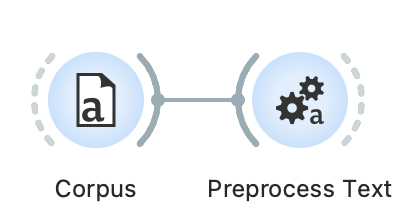
\includegraphics[width=0.9\linewidth]{workflow.png}
  \caption{}
\end{marginfigure}

\textit{Word Cloud} je preprosto prikazal vse besede in simbole, ki obstajajo v besedilu. Ampak običajno to ni to, kar hočemo. Ponavadi želimo prikazati zgolj pomenske enote, torej semantično bogate besede. Zato potrebujemo predprocesiranje.

\begin{figure*}[h]
  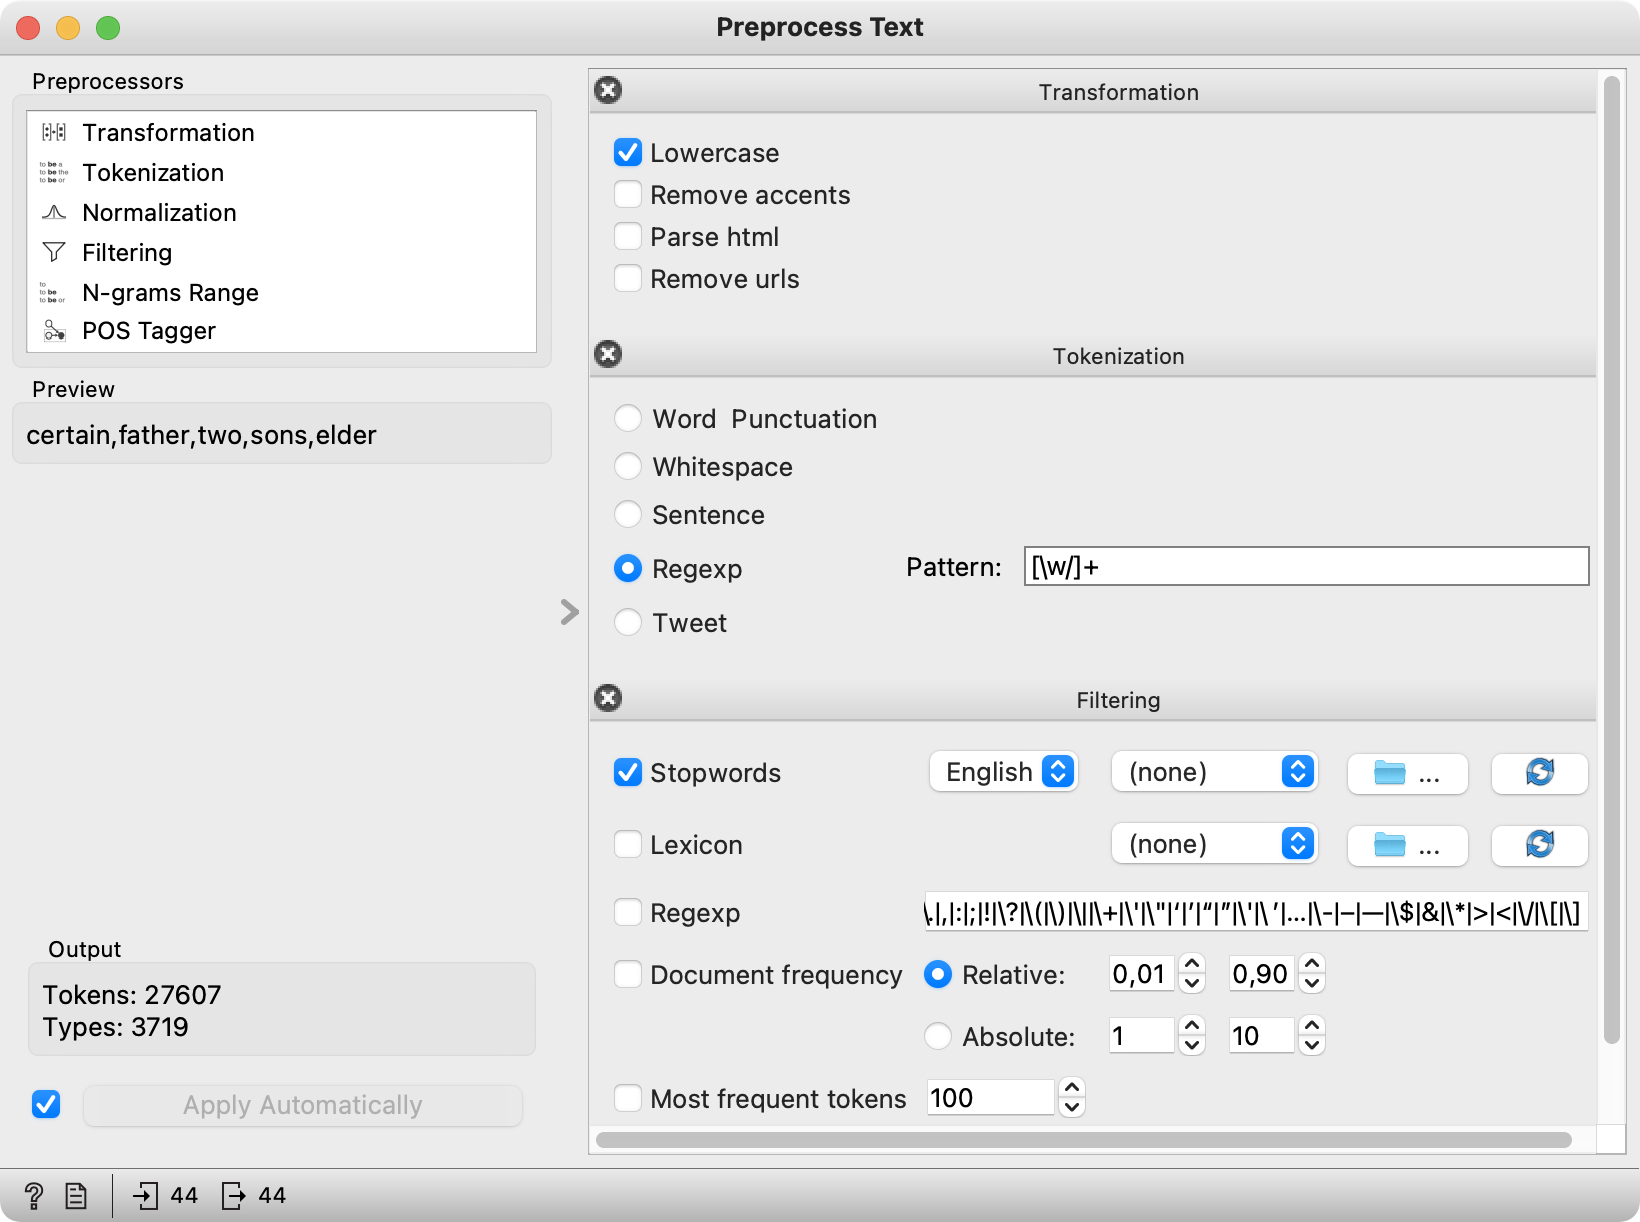
\includegraphics[width=\linewidth]{preprocess.png}%
  \caption{Preprocesiranje definira kaj je pomembno v podatkih. Je ``Zdravnik'' enako kot ``zdravnik''? Naj upoštevamo besede kot so ``in'', ``ali'', ``ko'' ali naj jih izpustimo? Ali želimo upoštevati besedi ``živel'' in ``živi'' kot isto besedo? Preprocesiranje definira osnovne enote analize.}
  \label{fig:002-preprocess}
\end{figure*}

V gradniku \widget{Preprocess Text} smo vse besede pretvorili v male črke, vsako besedo smo obravnavali kot svojo \textit{enoto (token)} in odstranili ločila, na koncu pa smo odstranili tudi nepomenske besede (npr. ‘in’, ‘da’, ‘čeprav’). Takšno predprocesiranje ustvari sledeče enote, ki jim pravimo tudi pojavnice:

\vspace{0.3cm}
\noindent ``To je vzorčni stavek.'' $\rightarrow$ ``vzorčni'', ``stavek''
\vspace{0.3cm}

Rezultate predprocesiranja si lahko pogledamo v gradniku \widget{Word Cloud}, kjer vidimo najpogostejše pojavnice. S to vizualizacijo lahko identificiramo odvečne besede in nepravilnosti.\marginnote{Pojavnica je osnovna enota naše analize. Lahko je beseda, besedna zveza, stavek … S predprocesiranjem definiramo osnovne enote za analizo.}

 \newpage

\begin{figure*}[h]
  \centering
  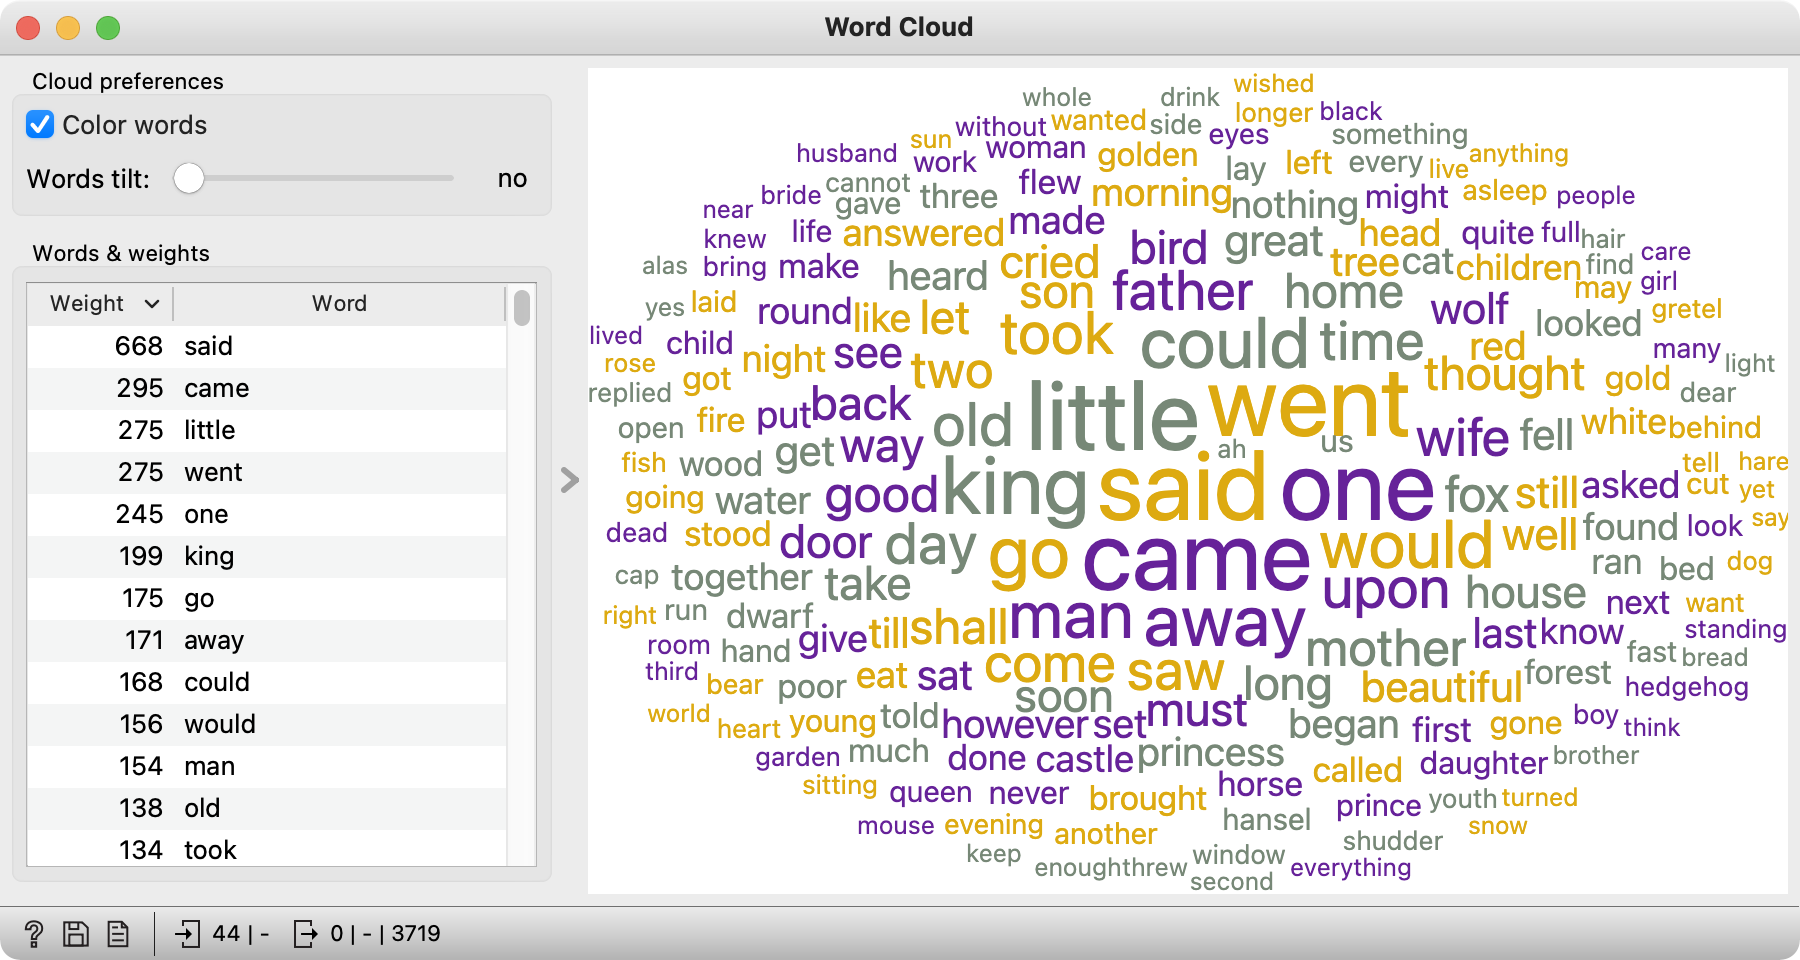
\includegraphics[width=\linewidth]{word-cloud.png}%
  \caption{Rezultate predprocesiranja vidimo v gradniku Word Cloud. Dve najpogostejši besedi sta “would” in “could”. Če se odločimo, da ti dve besedi nista primerni za našo analizo, ju moramo odstraniti. To lahko storimo s filtriranjem po meri.}
  \label{fig:002-word-cloud}
\end{figure*}

Ker ne želimo upoštevati besed brez pomena, smo že odstranili nekaj nepomenskih besed. Ampak morda generično filtriranje ni dovolj za našo analizo.

V tem primeru vedno lahko naložimo seznam besed po meri. Odprite urejevalnik besedil in ustvarite seznam nepomenskih besed oz. besed, ki jih želite odstraniti. Vsako besedo zapišite v svojo vrstico in shranite dokument v obliki \textit{.txt}.

\begin{figure}[h]
  \centering
  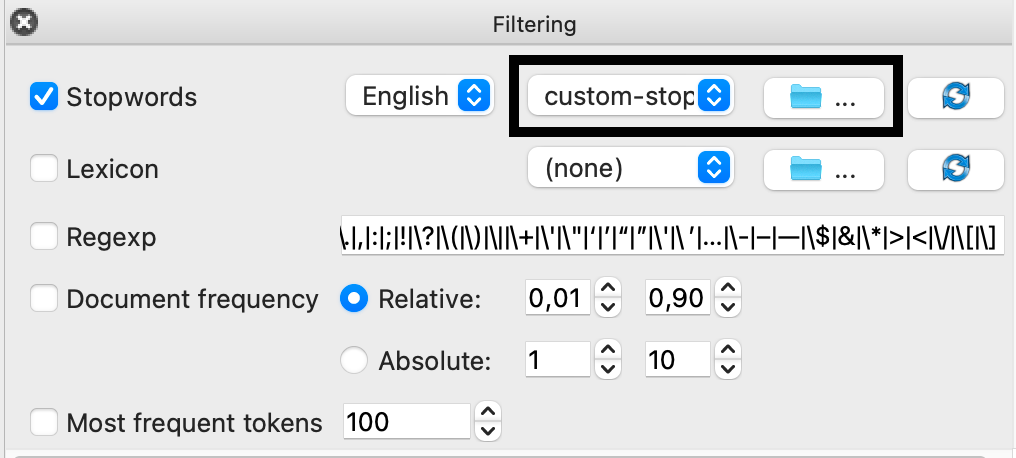
\includegraphics[width=\linewidth]{stop-words.png}%
  \caption{Dober urejevalnik besedil je Sublime, lahko pa uporabite tudi WordPad ali Word.}
  \label{fig:002-stop-words}
\end{figure}

Seznam besed naložite s klikom na ikono z mapo poleg opcije \textit{Stopwords} v razdelku \textit{Filtering}.

Filtriramo lahko tudi besede, ki so preredke ali prepogoste. Redke besede se pojavijo običajno le v nekaj dokumentih, medtem ko so prepogoste besede presplošne ali pa nimajo pomena (stopwords). Da bi ohranili le besede, ki zares predstavljajo naš korpus dokumentov, uporabimo filtriranje \textit{Document frequency} (Pogostost v besedilu). Če nastavimo vrednosti na 0,1 in 0,9, bomo obdržali le tiste besede, ki se pojavijo v več kot 10 \% in manj kot 90 \% dokumentov.

Predprocesiranje je ključ do uspešne analize besedil. Omenili smo le nekaj tehnik, sami pa lahko preizkusite še druge, na primer:

\begin{itemize}

\item \textit{normalizacija (Normalization)} pretvori vse besede v korene oz. osnovne oblike (na primer sinovi v sin)\marginnote{Pred kratkim smo za slovenščino dodali korenjenje z orodjema UDPipe in Lemmagen.}
\item \textit{n-grami} so večje enote, na primer bigrami (par zaporednih besed) in trigrami (trojke besed)
\item \textit{oblikoskladenjsko označevanje} (POS tagging)\marginnote{Za razlago POS oznak glejte:
http://nl.ijs.si/imp/msd/html-sl/} označi vsako enoto z njeno oblikoskladenjsko vlogo (sinovi $\rightarrow$ samostalnik, množina, oznaka = NNS)

\end{itemize}

\begin{figure}[h]
  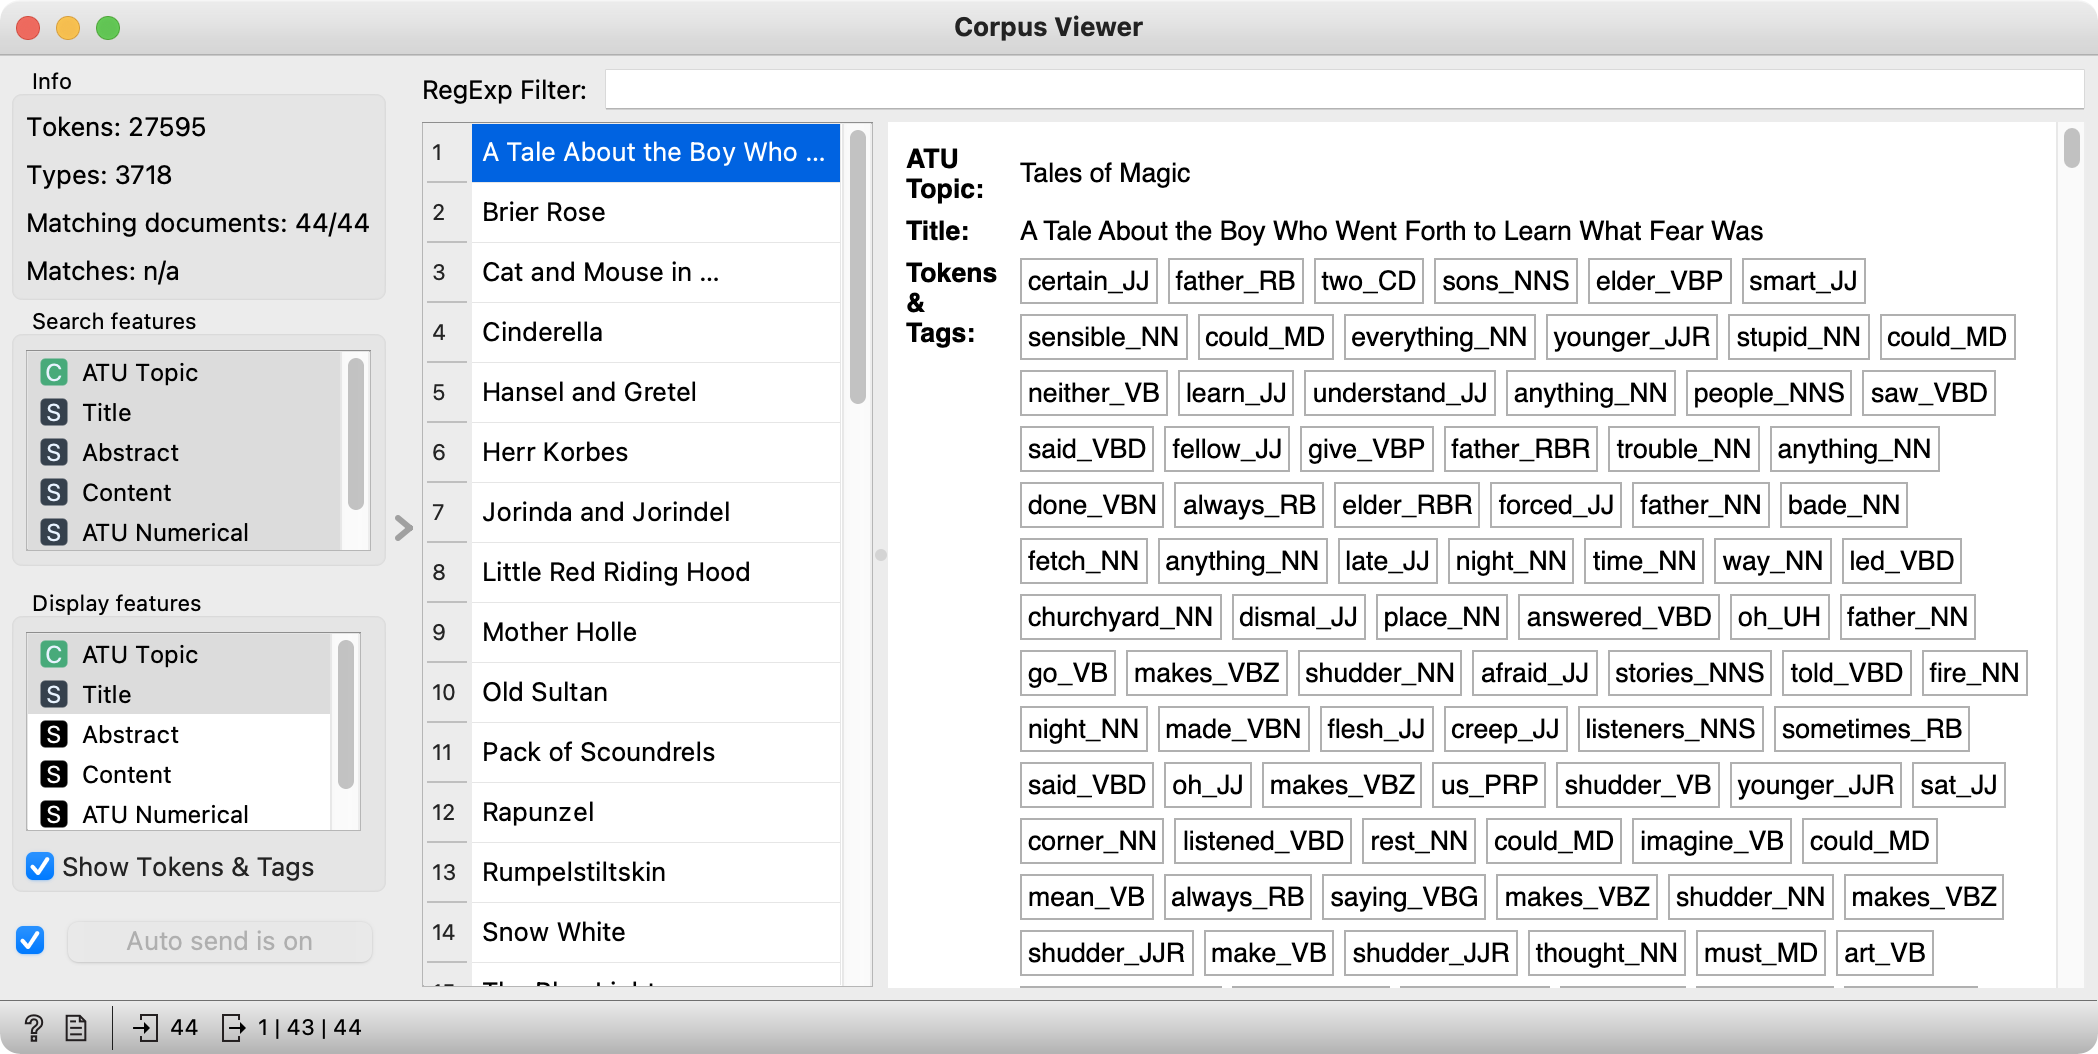
\includegraphics[width=\linewidth]{corpus-viewer-pos.png}%
  \caption{Na sliki vidite gradnik Corpus Viewer, s katerim si lahko pogledamo naslove, besedila dokumentov in pojavnice, na katere je predprocesiranje razbilo besedilo. V našem primeru imamo poleg pojavnic prikazane tudi POS oznake.}
  \label{fig:002-corpus-viewer-pos}
\end{figure}
